\documentclass[a4paper]{article}

\usepackage{graphicx}
\usepackage{multirow}
\usepackage{amsmath}
\usepackage{enumitem}
\usepackage{blindtext}
\usepackage{listings}
\usepackage{tikz}
\usetikzlibrary{automata,positioning,arrows}



\usepackage{xepersian}
\settextfont{B Roya}
\setlatintextfont{Tahoma}

\title{تمرین اول اتوماتا}
\author{نیما بهرنگ 96100114}
\date{\today}	
\begin{document}
\maketitle
\centering{استاد خزایی}


\section*{پرسش ۱}
\begin{enumerate}
\item{}
\begin{latin}
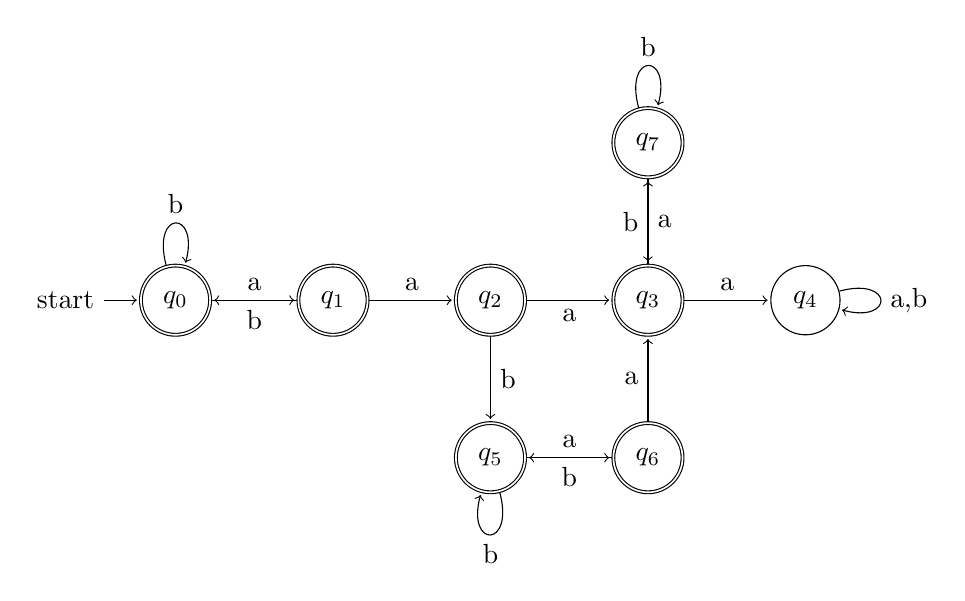
\begin{tikzpicture}[shorten >=1pt,node distance=2cm,on grid,auto] 
   \node[state,initial,accepting] (q0)   {$q_0$}; 
   \node[state,accepting] (q1) [right=of q0] {$q_1$}; 
   \node[state,accepting] (q2) [right=of q1] {$q_2$}; 
   \node[state,accepting] (q3) [right=of q2] {$q_3$}; 
   \node[state] (q4) [right=of q3] {$q_4$}; 
   \node[state,accepting] (q5) [below=of q2] {$q_5$}; 
   \node[state,accepting](q6) [below=of q3] {$q_6$};
   \node[state,accepting](q7) [above=of q3] {$q_7$};
    \path[->] 
(q0) edge  node {a} (q1)
	edge [loop above]node{b}()
(q1) edge  node  {b} (q0)
	edge node{a}(q2)
(q2) edge  node [swap] {a} (q3) 
	edge node {b} (q5)
(q3)edge  node {b} (q7)
	edge node{a}(q4)
(q4)edge [loop right] node{a,b}()
(q5)edge [loop below] node{b}()
	edge node{a}(q6)
(q6)edge node{a}(q3)
	edge node{b}(q5)
(q7)edge node{a}(q3)
	edge [loop above]node{b}();     
\end{tikzpicture}
\end{latin}

\item

\begin{latin}
\begin{tikzpicture}[shorten >=1pt,node distance=2cm,on grid,auto] 
   \node[state,initial] (u) [right=of q0] {$u$}; 
   \node[state] (s1) [above right=of u] {$s_1$}; 
   \node[state] (s2) [right=of s1] {$s_2$}; 
   \node[state] (s3) [right=of s2] {$s_3$}; 
   \node[state] (s4) [above right=of s3] {$s_4$}; 
   \node[state] (s5) [right=of s4] {$s_5$}; 
   \node[state] (s6) [below right=of s5] {$s_6$}; 
   \node[state] (t1) [below right=of u] {$t_1$}; 
   \node[state] (t2) [right=of t1] {$t_2$}; 
   \node[state] (t3) [right=of t2] {$t_3$}; 
   \node[state] (t4) [below right=of t3] {$t_4$}; 
   \node[state] (t5) [right=of t4] {$t_5$}; 
   \node[state] (t6) [above right=of t5] {$t_6$}; 
   \node[state,accepting](f) [above right=of t3] {$F$};
    \path[->] 
(u)edge node{a}(s1)
(u)edge node{b}(t1)
(s1)edge[loop above]node{a}()
(s1)edge node{b}(s2)
(t1)edge[loop below]node{b}()
(t1)edge node{a}(t2)
(s2)edge node{a}(s3)
(s2)edge node{b}(t1)
(t2)edge node{b}(t3)
(t2)edge node{a}(s1)
(s3)edge node{a}(s4)
(s3)edge node{b}(f)
(t3)edge node{b}(t4)
(t3)edge node{a}(f)
(s4)edge[loop above]node{a}()
(s4)edge node{b}(s5)
(s5)edge node{a}(s6)
(s5)edge[loop above] node{b}()
(s6)edge node{a}(s4)
(s6)edge node{b}(f)
(t4)edge[loop below]node{b}()
(t4)edge node{a}(t5)
(t5)edge node{b}(t6)
(t5)edge[loop below] node{a}()
(t6)edge node{b}(t4)
(t6)edge node{a}(f)
(f)edge[loop above]node{a,b}();
\end{tikzpicture}
\end{latin}

\item{}

\begin{latin}
\begin{tikzpicture}[shorten >=1pt,node distance=2cm,on grid,auto] 
   \node[state,initial, accepting] (u) [right=of q0] {$u$}; 
   \node[state] (s) [above right=of u] {$s$}; 
   \node[state,accepting](f) [below right=of u] {$F$};
    \path[->] 
(u)edge node{a}(s)
(u)edge[loop below] node{b}()
(s)edge[loop above]node{a}()
(s)edge node{b}(f)
(f)edge node{a}(s)
(f)edge node{b}(u);
\end{tikzpicture}
\end{latin}
\end{enumerate}
\section*{پرسش ۲}
\begin{enumerate}
\begin{latin}
\item{}

K = $a*b*$
\\
L = $b^*a(bb^*a)^*aa^*b$
\\
ans = $L(bL)^*aK^* $

\end{latin}
به زبان ساده تر همه رشته هایی که شامل زیررشته
\lr{aaba}
هستند
\item{}
\begin{latin}
J = $L(bL)^*a(aa^*b(bL)^*a)^*$
\\
ans = $J(bJ)^* $

\end{latin}
به زبان ساده تر همه رشته هایی که به
\lr{aaba}
ختم می شوند
\end{enumerate}

\section*{پرسش ۳}
\begin{enumerate}
\item{}

\lr{DFA} آن را این گونه می سازیم:\\
به تعداد
\lr{n+1}
استیت که به صورت متوالی با
\lr{a}
به هم متصل اند و اولی آنها حالت شروع است و آخرین این استیت ها فاینال است و به
\lr{p-۱}
استیت که به صورت مشابه با
\lr{a}
به صورت متوالی به یکدیگر وصل اند و آخرین آن ها نیز به آخرین استیت از دسته قبل وصل است
\\
\lr{DFA}
ساخته شده شامل کلماتی است که طول اولین آنها 
\lr{n}
بوده و سپس
\lr{p}
تا
\lr{p}
تا زیاد می شود
که همان تعریف تصاعدش است
\\
\begin{center}
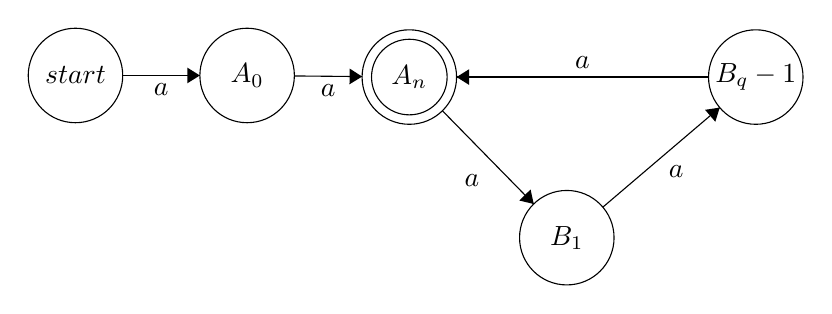
\begin{tikzpicture}[scale=0.2]
\tikzstyle{every node}+=[inner sep=0pt]
\draw [black] (10.5,-29) circle (3);
\draw (10.5,-29) node {$start$};
\draw [black] (21.4,-29) circle (3);
\draw (21.4,-29) node {$A_0$};
\draw [black] (31.7,-29.1) circle (3);
\draw (31.7,-29.1) node {$A_n$};
\draw [black] (31.7,-29.1) circle (2.4);
\draw [black] (41.7,-39.3) circle (3);
\draw (41.7,-39.3) node {$B_1$};
\draw [black] (53.7,-29.1) circle (3);
\draw (53.7,-29.1) node {$B_q-1$};
\draw [black] (13.5,-29) -- (18.4,-29);
\fill [black] (18.4,-29) -- (17.6,-28.5) -- (17.6,-29.5);
\draw (15.95,-29.5) node [below] {$a$};
\draw [black] (24.4,-29.03) -- (28.7,-29.07);
\fill [black] (28.7,-29.07) -- (27.91,-28.56) -- (27.9,-29.56);
\draw (26.55,-29.56) node [below] {$a$};
\draw [black] (33.8,-31.24) -- (39.6,-37.16);
\fill [black] (39.6,-37.16) -- (39.4,-36.24) -- (38.68,-36.94);
\draw (36.17,-35.67) node [left] {$a$};
\draw [black] (43.99,-37.36) -- (51.41,-31.04);
\fill [black] (51.41,-31.04) -- (50.48,-31.18) -- (51.13,-31.94);
\draw (48.65,-34.69) node [below] {$a$};
\draw [black] (50.7,-29.1) -- (34.7,-29.1);
\fill [black] (34.7,-29.1) -- (35.5,-29.6) -- (35.5,-28.6);
\draw (42.7,-28.6) node [above] {$a$};
\end{tikzpicture}
\end{center}

\item{}
برای
\lr{A} 
های متناهی می توان متناهی تصاعد حسابی با جمله اولیه هر عضو از
\lr{A}
و
\lr{p = 0}
ساخت\\
درجه هر استیت در
\lr{DFA}
متناظر آن حداکثر ۲ است
پس طبق قضایای گراف ساخته شده از تعدادی دور و تعدادی مسیر بی دور است
\\
چون 
\lr{DFA}
متناهی است پس به متناهی دور و مسیر افراز می شود
هر استیت شروع با هر استیت پایانی متشکل از یک مسیر است و استیت انتهایی آن دو حالت است
یکی این که دوری از حالت فاینال وجود داشته باشد که باز به حالت فاینال برسد ویا تشکیل مسیر دیگری دهد
\\
در حالت اول طول مسیر شروع تا فاینال٬ همان جمله اولیه تصاعد است که درصورتی که مسیری نباشد٬ صفر است
 و طول دور گفته شده همان اختلاف جملات است
 \\
 در حالت دوم هم تنها فرقش این است که طول دور صفر است یعنی اختلاف جملات همواره صفر است
 \\
 پس به تعداد ضرب تعداد فاینال ها در شروع ها که تعداد متناهی هستند
تصاعد٬ می توان 
\lr{S}
را ساخت
\end{enumerate}

\section*{پرسش ۵}
اگر دوتا دوتا حروف این کلمات را جدا کنیم تنها ۴ حالت زیر را دارند:
\\
\lr{aa, ab, ba, bb}\\
و جمع تعداد 
\lr{ab, ba}
های آنها فرد است پس در جایی یک
\lr{ab or ba}
آمده\\
سمت راست ترین آن را که فرض بگیریم :
\\
\lr{$*(ab + ba)(aa+bb)^*$}

حال قسمت قبل از آن باید تشکیل شده از زوج 
\lr{ab, ba}
باشد و باقی مهم نیستند یعنی:
\lr{$Z = (ab + ba)(aa+bb)^*$}
\lr{$L = (aa+bb)$}\\
\lr{$M = (ab+ba)$}\\
\lr{$ans = (L^*ML^*ML^*)^*Z$}

\section*{پرسش ۶}
\begin{enumerate}
\item{}
\begin{latin}
\begin{center}
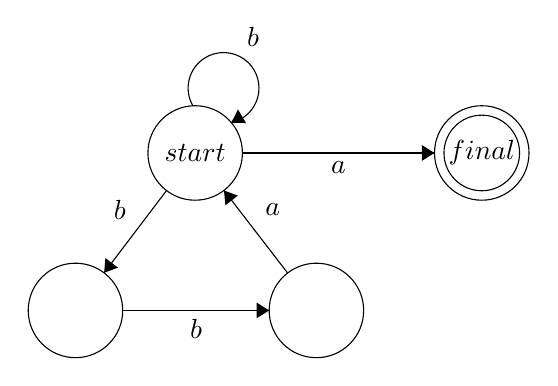
\begin{tikzpicture}[scale=0.2]
\tikzstyle{every node}+=[inner sep=0pt]
\draw [black] (20.9,-30.1) circle (3);
\draw (20.9,-30.1) node {$start$};
\draw [black] (39.1,-30.1) circle (3);
\draw (39.1,-30.1) node {$final$};
\draw [black] (39.1,-30.1) circle (2.4);
\draw [black] (13.3,-40.1) circle (3);
\draw [black] (28.6,-40.1) circle (3);
\draw [black] (23.9,-30.1) -- (36.1,-30.1);
\fill [black] (36.1,-30.1) -- (35.3,-29.6) -- (35.3,-30.6);
\draw (30,-30.6) node [below] {$a$};
\draw [black] (20.762,-27.115) arc (210.37062:-77.62938:2.25);
\draw (24.58,-23.4) node [above] {$b$};
\fill [black] (23.19,-28.18) -- (24.13,-28.2) -- (23.62,-27.34);
\draw [black] (19.08,-32.49) -- (15.12,-37.71);
\fill [black] (15.12,-37.71) -- (16,-37.38) -- (15.2,-36.77);
\draw (16.53,-33.7) node [left] {$b$};
\draw [black] (16.3,-40.1) -- (25.6,-40.1);
\fill [black] (25.6,-40.1) -- (24.8,-39.6) -- (24.8,-40.6);
\draw (20.95,-40.6) node [below] {$b$};
\draw [black] (26.77,-37.72) -- (22.73,-32.48);
\fill [black] (22.73,-32.48) -- (22.82,-33.42) -- (23.61,-32.81);
\draw (25.32,-33.69) node [right] {$a$};
\end{tikzpicture}
\end{center}
\end{latin}

\item{}
\begin{latin}

\begin{center}
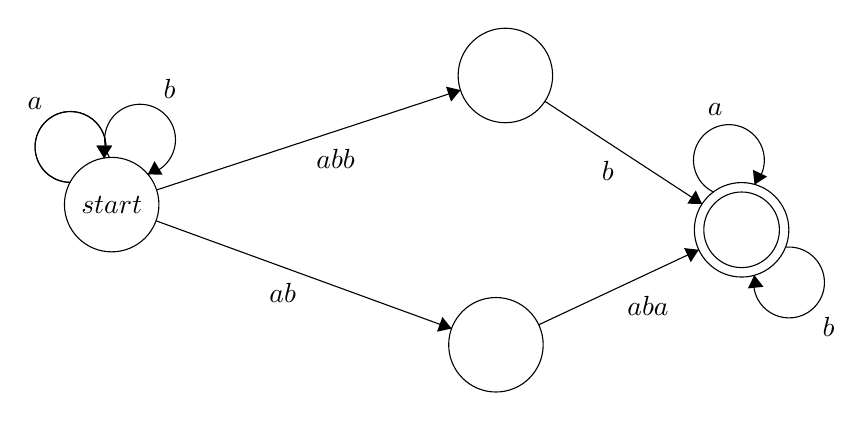
\begin{tikzpicture}[scale=0.2]
\tikzstyle{every node}+=[inner sep=0pt]
\draw [black] (11.7,-36.6) circle (3);
\draw (11.7,-36.6) node {$start$};
\draw [black] (36.7,-28.4) circle (3);
\draw [black] (36.1,-45.5) circle (3);
\draw [black] (51.7,-38.2) circle (3);
\draw [black] (51.7,-38.2) circle (2.4);
\draw [black] (14.55,-35.67) -- (33.85,-29.33);
\fill [black] (33.85,-29.33) -- (32.93,-29.11) -- (33.25,-30.06);
\draw (25.92,-33.07) node [below] {$abb$};
\draw [black] (11.562,-33.615) arc (210.37062:-77.62938:2.25);
\draw (15.38,-29.9) node [above] {$b$};
\fill [black] (13.99,-34.68) -- (14.93,-34.7) -- (14.42,-33.84);
\draw [black] (9.066,-35.188) arc (269.53768:-18.46232:2.25);
\draw (6.83,-30.61) node [above] {$a$};
\fill [black] (11.22,-33.65) -- (11.73,-32.85) -- (10.73,-32.85);
\draw [black] (9.066,-35.188) arc (269.53768:-18.46232:2.25);
\fill [black] (11.22,-33.65) -- (11.73,-32.85) -- (10.73,-32.85);
\draw [black] (54.476,-39.307) arc (95.98721:-192.01279:2.25);
\draw (57.23,-43.71) node [below] {$b$};
\fill [black] (52.51,-41.08) -- (52.1,-41.92) -- (53.09,-41.82);
\draw [black] (49.919,-35.8) arc (244.30485:-43.69515:2.25);
\draw (50.03,-30.97) node [above] {$a$};
\fill [black] (52.52,-35.33) -- (53.32,-34.82) -- (52.42,-34.39);
\draw [black] (39.21,-30.04) -- (49.19,-36.56);
\fill [black] (49.19,-36.56) -- (48.79,-35.7) -- (48.25,-36.54);
\draw (43.2,-33.8) node [below] {$b$};
\draw [black] (38.82,-44.23) -- (48.98,-39.47);
\fill [black] (48.98,-39.47) -- (48.05,-39.36) -- (48.47,-40.26);
\draw (45.76,-42.36) node [below] {$aba$};
\draw [black] (14.52,-37.63) -- (33.28,-44.47);
\fill [black] (33.28,-44.47) -- (32.7,-43.73) -- (32.36,-44.67);
\draw (22.56,-41.59) node [below] {$ab$};
\end{tikzpicture}
\end{center}
\end{latin}

\end{enumerate}

\section*{پرسش ۷}
\lr{$abab(baa+ababb)^*$}
چون انتهای تمام رشته های زبان اول با 
\lr{baba}
تمام می شد پس وارونه آنها با 
\lr{abab}
شروع می شود و
\\
\lr{L = (aab)}
\\
\lr{M = (bbaba)}
\\
چون زبان ساخته شده از تعدادی
\lr{M, L}
 است
وارونه هر کلمه آن ساخته شده از تعدادی وارونه 
\lr{M, L}
 است
پس مجموعه همه وارونه ها
\lr{,}
 وارونه مجموعه همه \lr{M, L} هاست

\section*{پرسش۸}
$\lambda = \lambda\lambda \Rightarrow f(\lambda) = f(\lambda\lambda) $
\\
$f(\lambda\lambda) = f(\lambda)f(\lambda) \Rightarrow f(\lambda) = f(\lambda)f(\lambda) \Rightarrow$
\\
$f(\lambda) = \lambda$

\section*{پرسش ۱۰}
\begin{enumerate}
\begin{latin}
\item{}
\item{}
\item{}
\item{}
$(b + a(ba^*bb)^*(a + ba^*ba))^*$
\end{latin}
\end{enumerate}

\end{document}